\documentclass[journal, a4paper]{IEEEtran}
\usepackage[italian]{babel}
\usepackage{booktabs}
\usepackage{siunitx}%Questo serve a caricare il pacchetto delle unità di misura del sistema internazionale%
\usepackage[utf8]{inputenc}
\usepackage{graphicx} 
\usepackage{url}
\usepackage{amsmath}
\usepackage{amssymb}


\usepackage{keyval}
\usepackage{xcolor}
\usepackage{caption}
\usepackage{subfig}
\usepackage{tikz}
\usepackage{circuitikz}
\usepackage{authblk}
%\usepackage{hyperref}

\begin{document}


% Define document title and author
	\title{Tecnologie Digitali - Logbook Week 13}
	\author[1]{Salvatore Bottaro}
		\author[2]{Lorenzo M. Perrone}
		\affil[1]{\texttt{salvo.bottaro@hotmail.it}}
		\affil[2]{\texttt{lorenzo.perrone.lmp@gmail.com}}
	\markboth{Tecnologie Digitali - Di Lieto}{}
	\maketitle
	
\begin{abstract}
	Logbook di laboratorio di Tecnologie Digitali, a.a. 2015/2016. Week 13
\end{abstract}

\section{Ritardo dei segnali}
Un fattore che è entrato solo marginalmente nella discussione della precedente esperienza (in particolare nella sezione dei contatori sincroni e asincroni) è il tempo di ritardo tipico di una porta \textsc{CMOS}. Per essere più precisi, come si rileva dal datasheet del \textsc{MC14011B} \textbf{NAND}, esistono diversi tempi caratteristici tipici di un integrato (vedi Figura ()): noi in particolare siamo interessati a quello che è definito \textit{propagation delay time}, $t_{PLH}$ o $t_{PHL}$, vale a dire il tempo che impiega l'output del circuito a passare da \textsc{high} $\rightarrow$ \textsc{low} (o viceversa) non appena viene ricevuto in input un fronte d'onda opportuno. Nella seguente tabella vengono riportati i valori tipici di questi tempi per diverse tensioni di alimentazione.\\


\begin{table}
\centering
\caption{Caratteristiche del 14011}
\label{tab:data}
\begin{tabular}{c|cl|c}
  \hline
  \textbf{Delay time} & $V_{DD}$ (V)& \textbf{Valore typ} (ns)& \textbf{Valore max} (ns) \\
  \hline 
            &  5  & 100 &  200  \\ \cline{2-3}
  $t_{TLH}$ & 10  & 50 &  100   \\ \cline{2-3}
            & 15  & 40 &   80   \\
  \hline 
            &  5  & 100 &  200  \\ \cline{2-3}
  $t_{THL}$ & 10  & 50 &  100   \\ \cline{2-3}
            & 15  & 40 &   80   \\
  \hline
  $t_{PLH}$, &  5  & 125 &  250   \\ \cline{2-3}
  $t_{PHL}$  & 10  & 50 &   100   \\ \cline{2-3}
             & 15  & 40 &   80   \\
  \hline
\end{tabular}
\end{table}
~\\

Un modo per valutare sperimentalmente i tempi di ritardo dei \textbf{NAND} è quello di sfruttare un circuito costruito come in Figura (\ref{fig:es2_circuit}). Il funzionamento è facile da intuire: un ingresso dell'\textbf{AND} riceve il segnale di \textsc{clk}, il secondo riceve il suo negato (mediante un numero dispari di \textbf{NOT} che nel nostro caso sono ottenuti ciascuno tramite un \textbf{NAND} cortocircuitato agli ingressi). Se non vi fossero tempi di ritardo di alcun tipo l'output del circuito sarebbe banalmente sempre \textsc{low}. \\
In realtà, grazie al \textit{propagation delay time} il segnale negato non giunge in maniera sincrona con quello di clock agli ingressi dell'\textbf{AND}, ma leggermente sfasato (ci sono due differenti regimi da approfondire, e cioè cosa succede quando il tempo di ritardo è inferiore al semiperiodo e quando è invece superiore; per adesso ci concentriamo sul primo caso), e ciò permette che per un certo $\Delta t$ l'uscita sia \textsc{high}: come si vede anche dalla Figura (\ref{fig:delay1}), il duty-cycle dell'output è proprio una misura del ritardo dovuto ai tre \textbf{NOT}, in particolare $\Delta t = \eta \, T$, e noi possiamo utilizzare il VI \textsc{contatore\_pulsew} per misurare il \textsc{rising-time}.\\



\begin{figure}
\centering
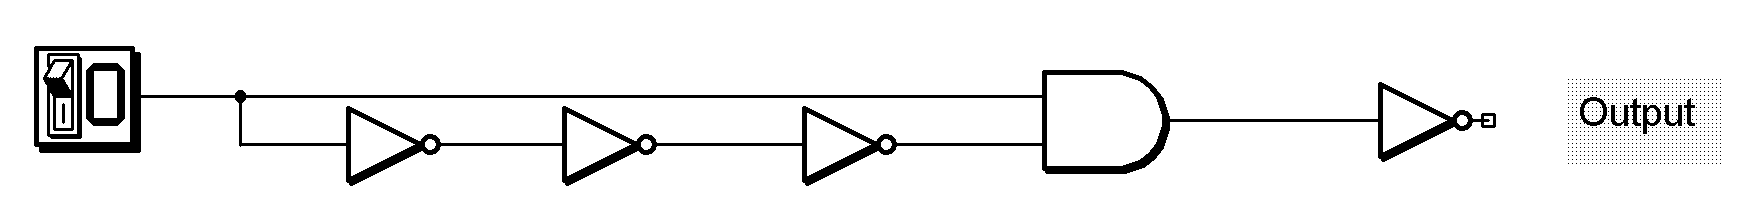
\includegraphics[width=0.7\linewidth]{./es2_circuit}
\caption{Circuito per valutare il delay dei segnali}
\label{fig:es2_circuit}
\end{figure}

\begin{figure}
\centering
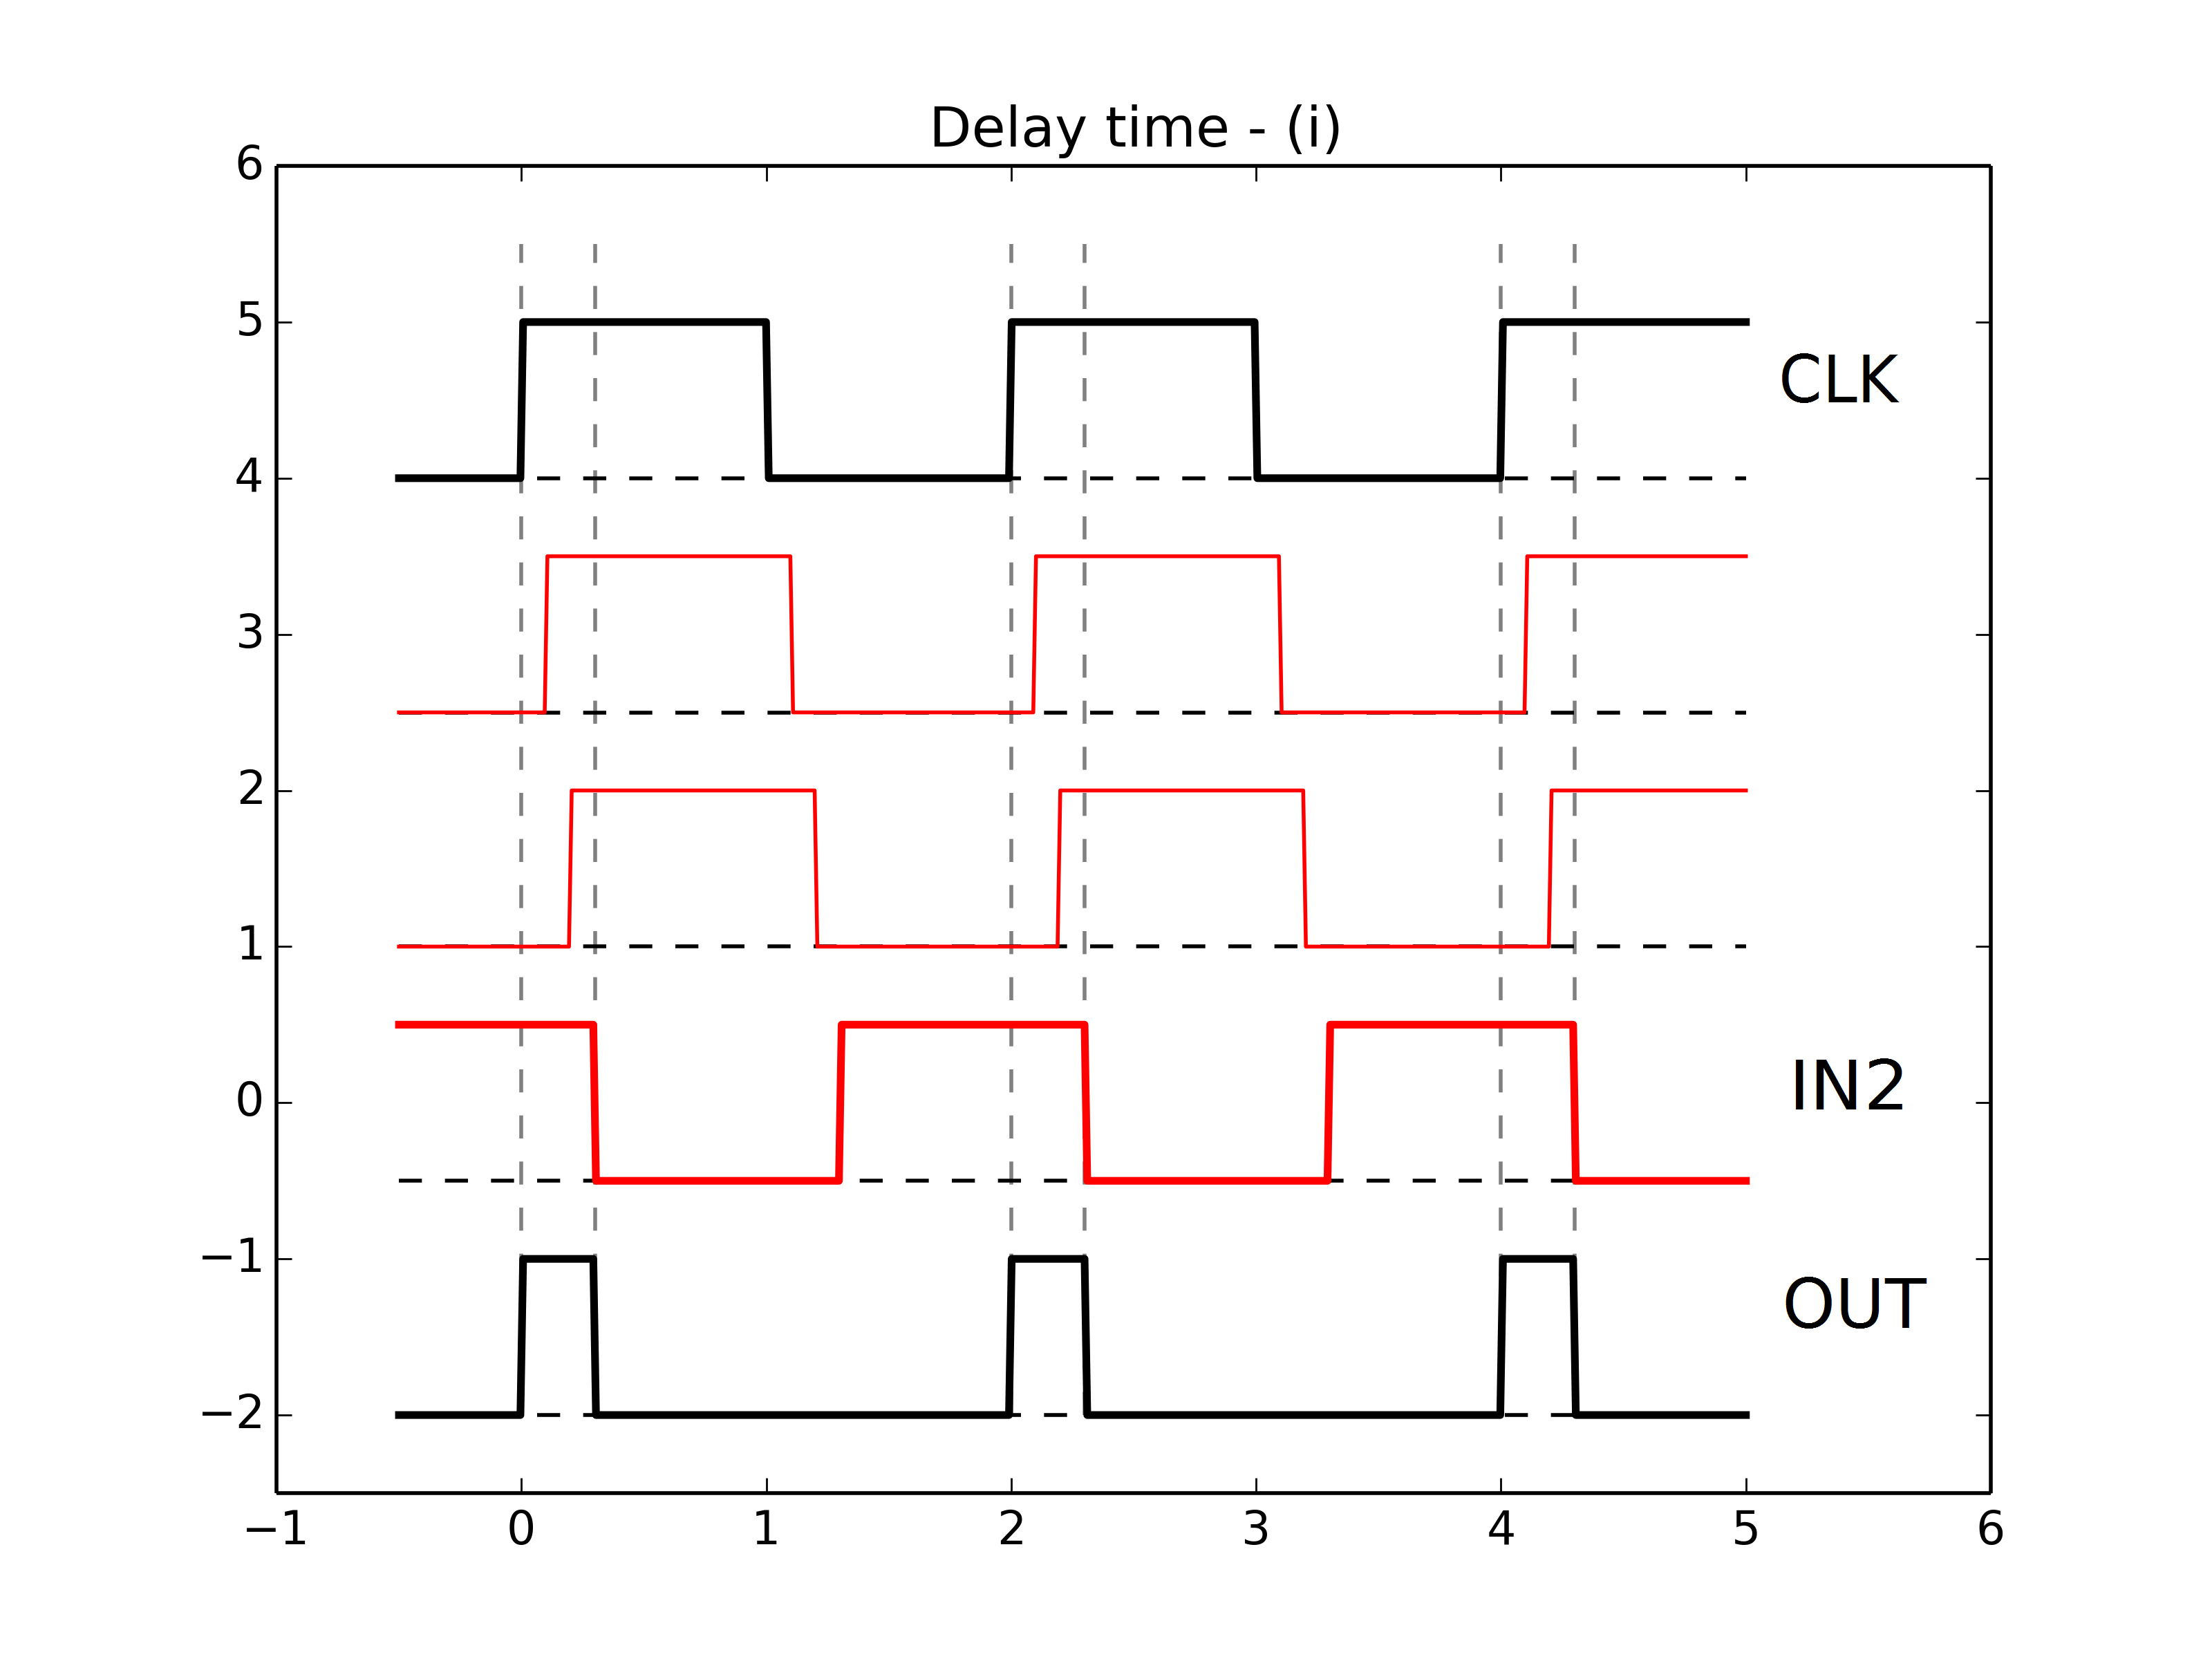
\includegraphics[width=0.7\linewidth]{./delay1}
\caption{Delay time - semiperiodo maggiore del ritardo}
\label{fig:delay1}
\end{figure}


Per esaminare il caso in cui il ritardo del ramo \textbf{NOT} supera il semiperiodo è sufficiente ragionare in questo modo: quando il ritardo è arrivato a misurare esattamente un semiperiodo, il segnale è come shiftato di $\pi$ che, nel caso di segnale logico a onda quadra, equivale a negarlo. Nel ramo inferiore ci sarebbero quindi 2 \textbf{NOT} e l'\textbf{AND} di \textsc{CLK} con NOT(NOT(CLK)) è ovviamente sempre 1. Seguendo un ragionamento simmetrico rispetto al caso precedente, non aappena il ritardo avrà superato il semiperiodo, questo sarà evidente come un impulso negativo nell'output del circuito e questa volta andrà misurato dunque il \textsc{falling-time} (vedi anche Figura (\ref{fig:delay2})).\\ 

\begin{figure}
\centering
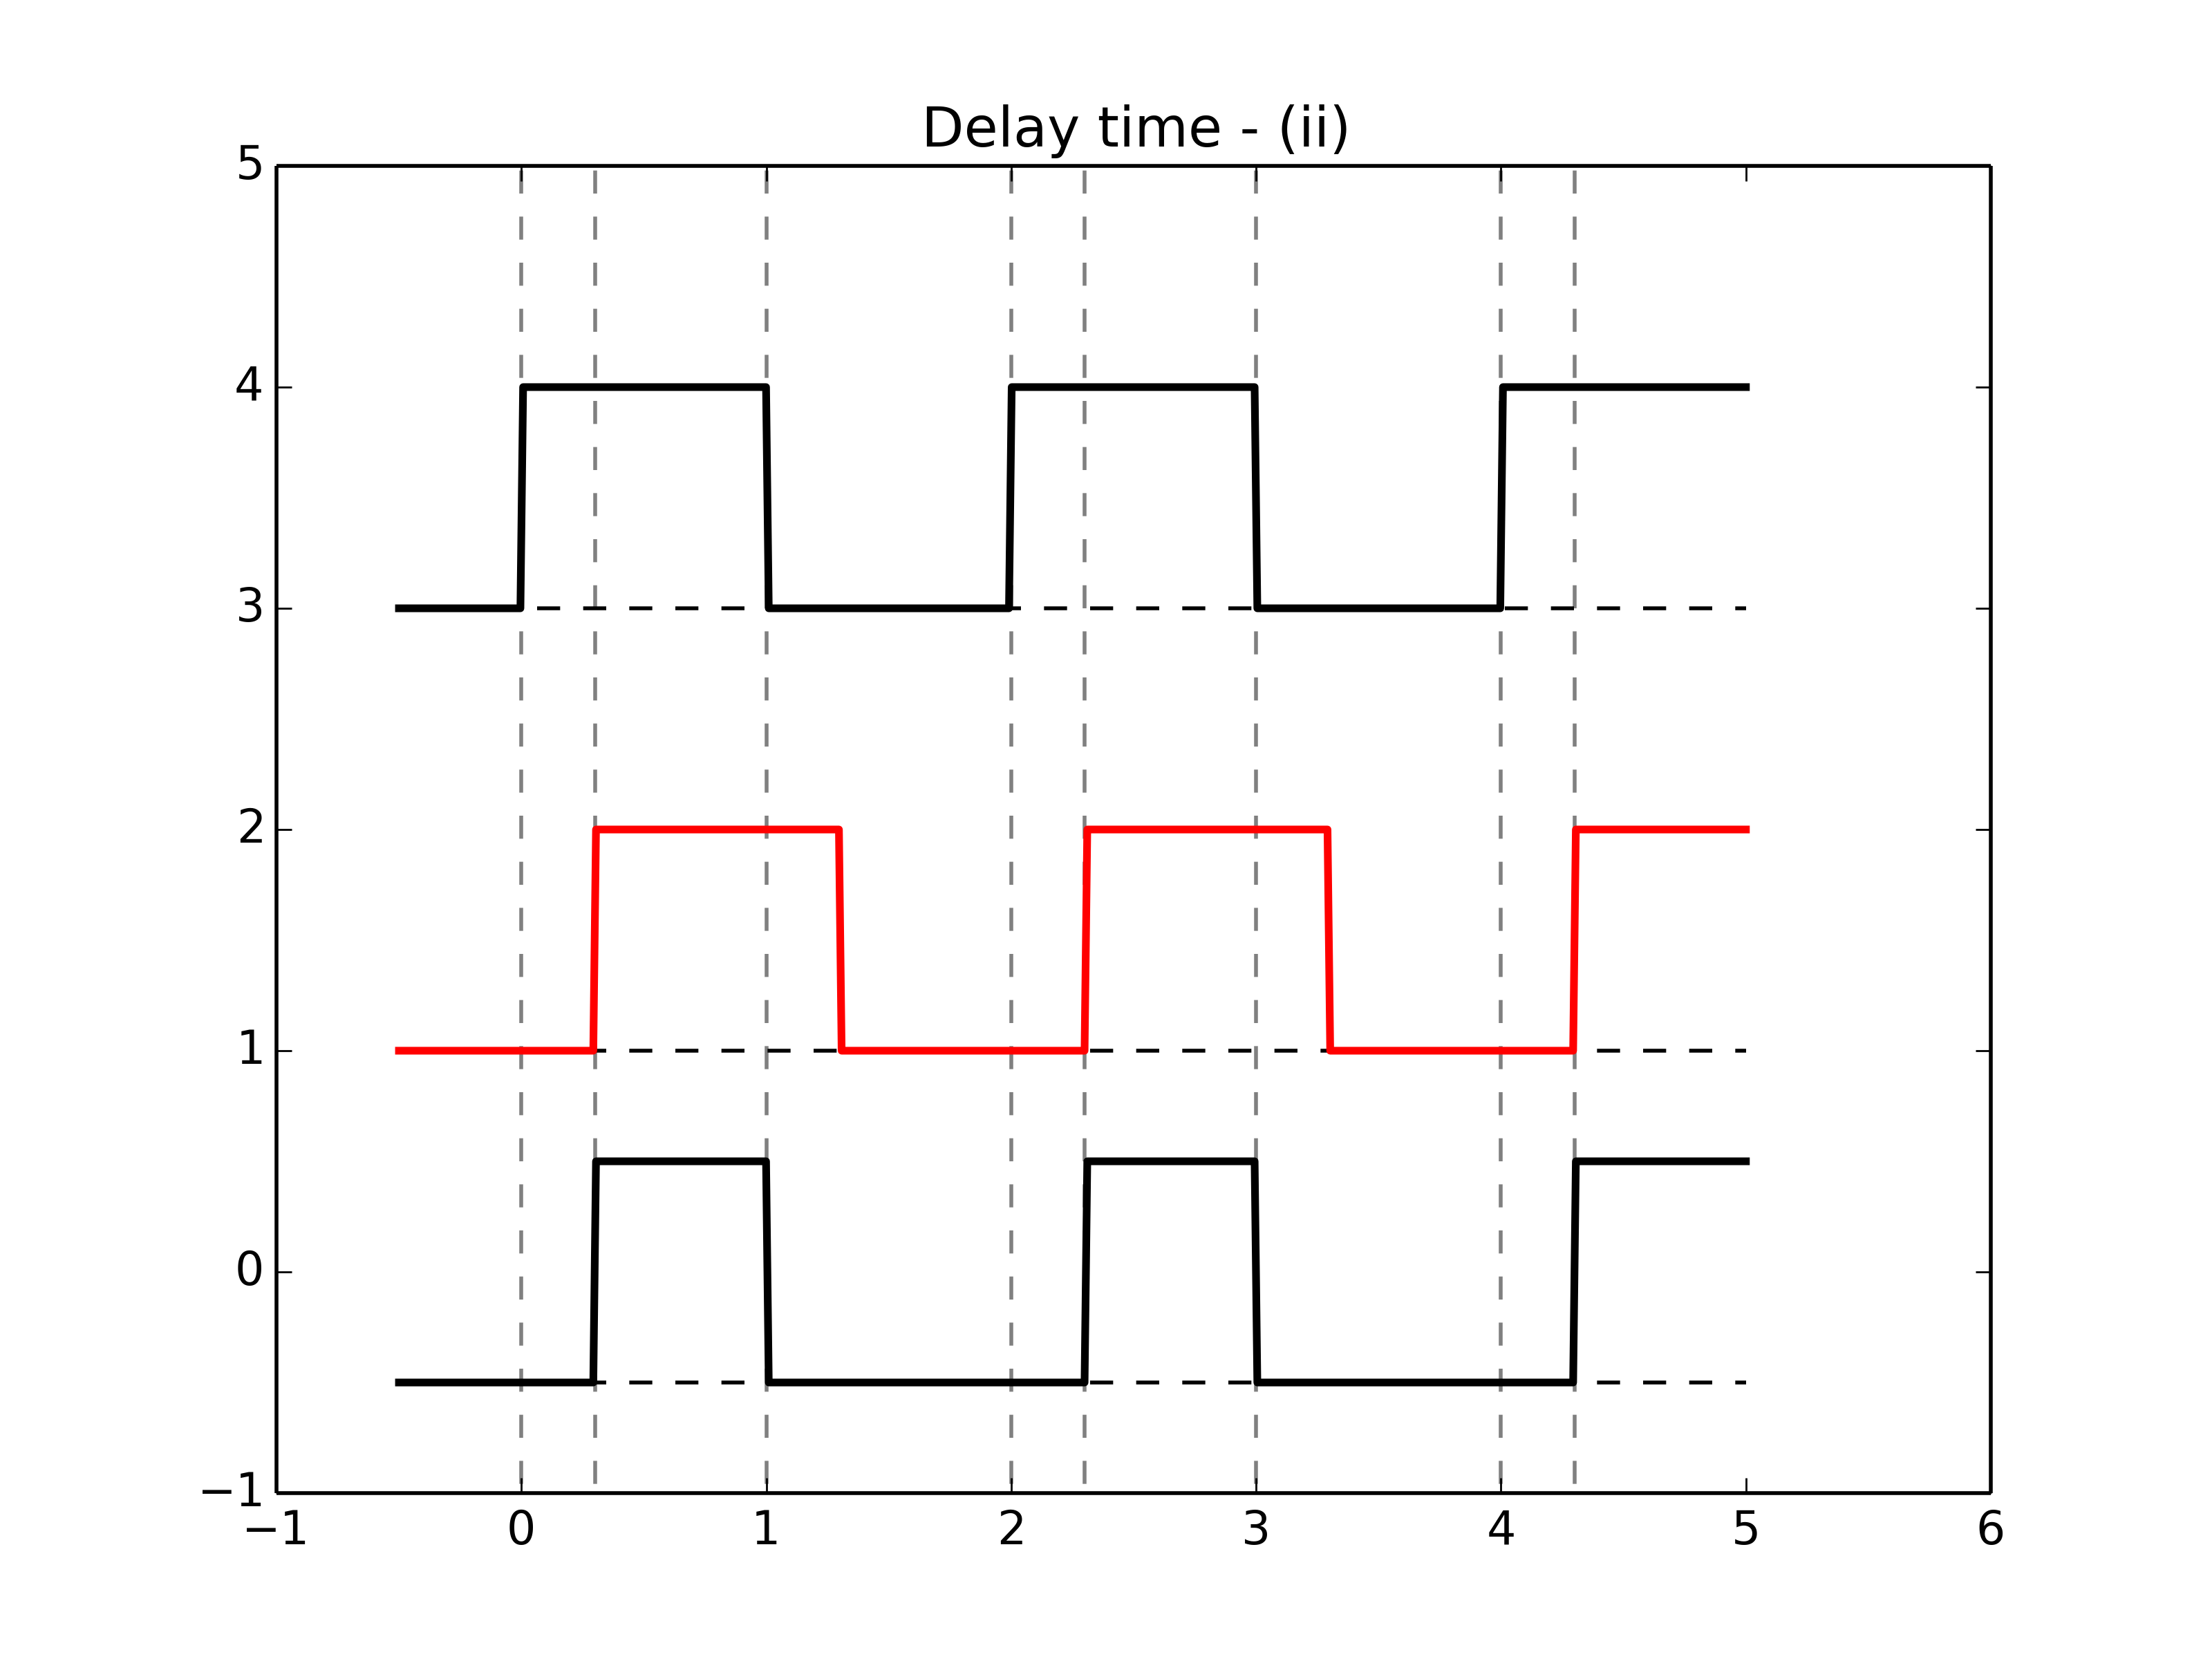
\includegraphics[width=0.7\linewidth]{./delay2}
\caption{Delay time - ritardo maggiore del semiperiodo}
\label{fig:delay2}
\end{figure}


Prima di verificare effettivamente le nostre ipotesi è necessario però tener conto del fatto che il segnale di uscita di un tale circuito tende ad essere piuttosto sporco: ciò è dovuto al fatto che il delay accumulato a valle dei tre \textbf{NOT} è confrontabile con i tempi di risalita e di discesa della tensione (quelli che nel datasheet vengono indicati con $t_{THL}$ e $t_{TLH}$) e ciò rende estremamente difficoltoso, se non impossibile, per il \textsc{contatore\_pulsew} dare dei buoni risultati poichè quest'ultimo, non appena vede un segnale poco al di sopra del valore \textsc{low}, inizia a misurare il suo rising time mentre invece il fronte d'onda vero e proprio deve ancora arrivare.\\
Per ovviare a questo inconveniente, è prassi cercare di "ripulire" il segnale ponendo in serie un'altra porta (noi abbiamo scelto un \textbf{NOT}) con dei livelli \textsc{high} e \textsc{low} in uscita ben definiti. In questo caso, ovviamente, il delay sarà dato dal falling time.\\

  
Realizziamo quindi il circuito: ci aspettiamo un delay di qualche centinaia di ns, per cui scegliamo una frequenza di clock di 100kHz (in modo che il semiperiodo risulti maggiore del delay), il segnale è di 5$V_{PP}$ con un offset di $2.5V$, e l'output del circuito (\textbf{NOT} incluso) è collegato alla \textsc{CB3} per poterlo analizzare con l'apposito VI. Facendo una media fra i campionamenti del \textsc{contatore\_pulsew} e calcolando lo scarto quadratico medio, otteniamo il valore di $t_D = 97(2) ns$, piuttosto contenuto se consideriamo i tempi tipici di propagazione riportati sul datasheet, ma in linea con quanto ottenuto dagli altri gruppi.

\section{Circuiti monostabili}
Tutti i circuiti esaminati fino ad ora sono essenzialmente \textit{stabili}, in particolare i flip-flop sono anche chiamati \textit{bistabili}. Andiamo ora ad esaminare i cosiddetti circuiti \textbf{monostabili} caratterizzati da uno stato in cui possono permanere per un tempo indefinito fino a quando non ricevono un impulso opportuno (di salita o di discesa) a cui segue una fase di transizione dalla durata regolabile, dovuta al processo di carica e scarica di un condensatore. \\
Noi useremo un circuito monostabile impiegato per produrre degli impulsi in uscita dalla durata programmabile. Fra le caratteristiche proprie di circuti di questo tipo vi sono: la modalità di trigger (come già detto), la possibilità di retrigger, cioè nel nostro caso la capacità di produrre un secondo impulso mentre è ancora attivo il primo, e quella di reset.\\
Il circuito monostabile è riportato in Figura ().\\

Per identificare lo stato stabile ci viene suggerito di considerare il condensatore scarico e il ramo U1-C scollegato. Con l'ingresso T nello stato \textsc{low} gli stati del circuito sono come riportato nella tabella che segue (V1 è a terra in questa configurazione):\\


\begin{table}
\centering
\caption{tab\_es3}
\label{tab:es3}
\begin{tabular}{c|cl|c}
  \hline
  \textbf{T} & \textbf{U1} & \textbf{V1} & \textbf{U2} \\
  0 & 1 & 0 & 1
\end{tabular}
\end{table}
~\\

Se adesso ripristiniamo il collegamento U1-C si ha che il piatto di sinistra del condensatore passa immediatamente a 5V: a causa dell'istantaneità di questo processo non si può accumulare carica su alcuna delle armature del condensatore, per cui la differenza di potenziale fra queste deve rimanere costante ($C \Delta V = Q$), e ciò implica che anche V1 si troverà istantaneamente a 5V (valore logico \textsc{high}). L'uscita U2 passa dunque a 0, il che implica che qualunque sia il valore di T, U1 rimane a 1. La situazione istantanea (t = 0) è riassunta come segue (X = doesn't matter):\\

\begin{table}
\centering
\caption{tab\_es3bis}
\label{tab:es3bis}
\begin{tabular}{c|cl|c}
  \hline
  \textbf{T} & \textbf{U1} & \textbf{V1} & \textbf{U2} \\
  X & 1 & 1 & 0
\end{tabular}
\end{table}
~\\

Tuttavia ci rendiamo immediatamente conto che questa è una situazione che non è per nulla stabile, in quanto l'armatura destra del condensatore è collegata a terra mediante una resistenza: da terra risalgono delle caariche negative e la tensione V1 via via decresce seguendo l'andamento esponenziale tipico del processo di scarica di un condensatore. Le uscite rimangono inalterate fino a quando la tensione V1 non scende al di sotto della linea di demarcazione di valore logico \textsc{low}. A questo punto U2 torna a 1, se T è nel frattempo tornato \textsc{high} allora U1 scende a \textsc{low}, il che implica che V1, per mantenere costante la differenza di potenziale ai capi delle piastre del condensatore, scende a sua volta a circa -5V, che tuttavia viene letto come segnale logico ancora \textsc{low} e le uscite non cambiano. Quando V1 si sarà caricato fino a 0V saremo ritornati nella situazione stazionaria di partenza. Se invece, quando U2 sale a 1 T è ancora \textsc{low}, allora U1 continua a rimanere 1 e V1 a calare fino a quando non arriva un fronte di risalita su T: a questo punto il sistema evolve nello stesso modo del caso precedente. L'intera sequenza è riassunta in Figura ().\\


La costante di tempo nominale che caratterizza la carica del condensatore (e quindi la durata dell'impulso U2 in uscita) è definita come $\tau_s = 0.7 \, RC$. Siamo interessati a misurare proprio questo tempo caratteristico, ma prima verifichiamo che il circuito funzioni come previsto collegando il trigger (comandato dalla \textsc{cb47}) e l'uscita U2 al tester digitale. Le connessioni sono state fatte come in Figura (). Per iniziare abbiamo scelto una combinazione RC di (149.8(1)k$\Omega$, 1 $\mu$F), in modo da avere una $\tau_s$ di $\sim$ 0.1s.\\

Si nota effettivamente un rapido impulso (negativo) di U2 compatibile con una durata di un decimo di secondo. Abbiamo fattoulteriori prove cambiando le resistenze e spingendoci fino a 10M$\Omega$: in quest'ultimo caso l'impulso negativo dura circa 5s, un valore vicino a quello previsto di $\sim$7s, e comunque piuttosto divertente da osservare. \\
Un'altra interessante osservazione risulta dallo strano comportamento che si ottiene quando ci cerca di osservare contemporaneamente col tester digitale T, V1 e U2, dove nel caso di V1 si vorrebbe visualizzare almeno qualitativamente la diminuzione dell'intensità luminosa del LED come conseguenza della caduta esponenziale di V1: quando tutte e tre le porte sono collegate al tester digitale si riesce effettivamente ad osservare l'affievolimento del LED corrispondente a V1 ma manca completamente qualunque impulso su U2, anche brevissimo e anche utilizzando resistenze da diversi M$\Omega$. Poichè ovviamente V1 e U2 non sono variabili quantistiche incompatibili, siamo andati a ricercare la causa di questo insolito comportamento nella perturbazione introdotta dal LED fra V1 e gli ingressi di U2: probabilmente a causa della bassa resistenza del LED la corrente tende a passare attraverso quest'ultimo invece che su R (e soprattutto arrivare a U2)e gli ingressi di U2 risultano letti sempre come \textsc{low}, un po' come se fosse cortocircuitato il ramo fra V1 e U2.\\

Analizziamo ora più in dettaglio i quattro segnali del circuito registrandoli con \textsc{acquis\_base4}, campionando a 1kS/s tutti e quattro i canali per una durata di 3sall'interno dei quali abbiamo dato manualmente l'impulso negativo di T. Il \textsc{CLK} è stato collegato alla \textsc{cb68}, U2 alla \textsc{cb33}, U1 alla \textsc{cb65}, V1 alla \textsc{cb30}.\\
Il grafico per la resistenza da 150k$\Omega$ è riportato in Figura (\ref{fig:es6_150k}). Come si vede dal grafico, ci troviamo nella situazione in cui quando U2 ha terminato il suo impulso negativo, T non è ancora risalito, per cui V1 continua a decrescere esponenzialmente. Non appena viene riportato a 1 T1 allora anche U1 (in verde) risale, V1 scende improvvisamente al di sotto di 0V, tuttavia non raggiunge una tensione di circa -5V, come aspettato, ma si ferma a -0.65V, pensiamo a causa della protezione che hanno gli ingressi dei \textbf{NAND} e che evitano che in ingresso vengano ricevute tensioni di molto inferiori allo zero (sul datasheet è riportata una tensione minima accettata di -0.5V).\\
Se andiamo a stimare dai campionamenti la durata dell'impulso $\tau_s$ otteniamo un valore di 78(1)ms, non molto distante da quello previsto di $\sim 0.105s$. Inoltre, il livello di tensione sotto il quale V1 viene considerato come \textsc{low} è di 2.85(2), estremamente vicino al valore tipico di 2.75V segnalato sul datasheet.

\begin{figure}
\centering
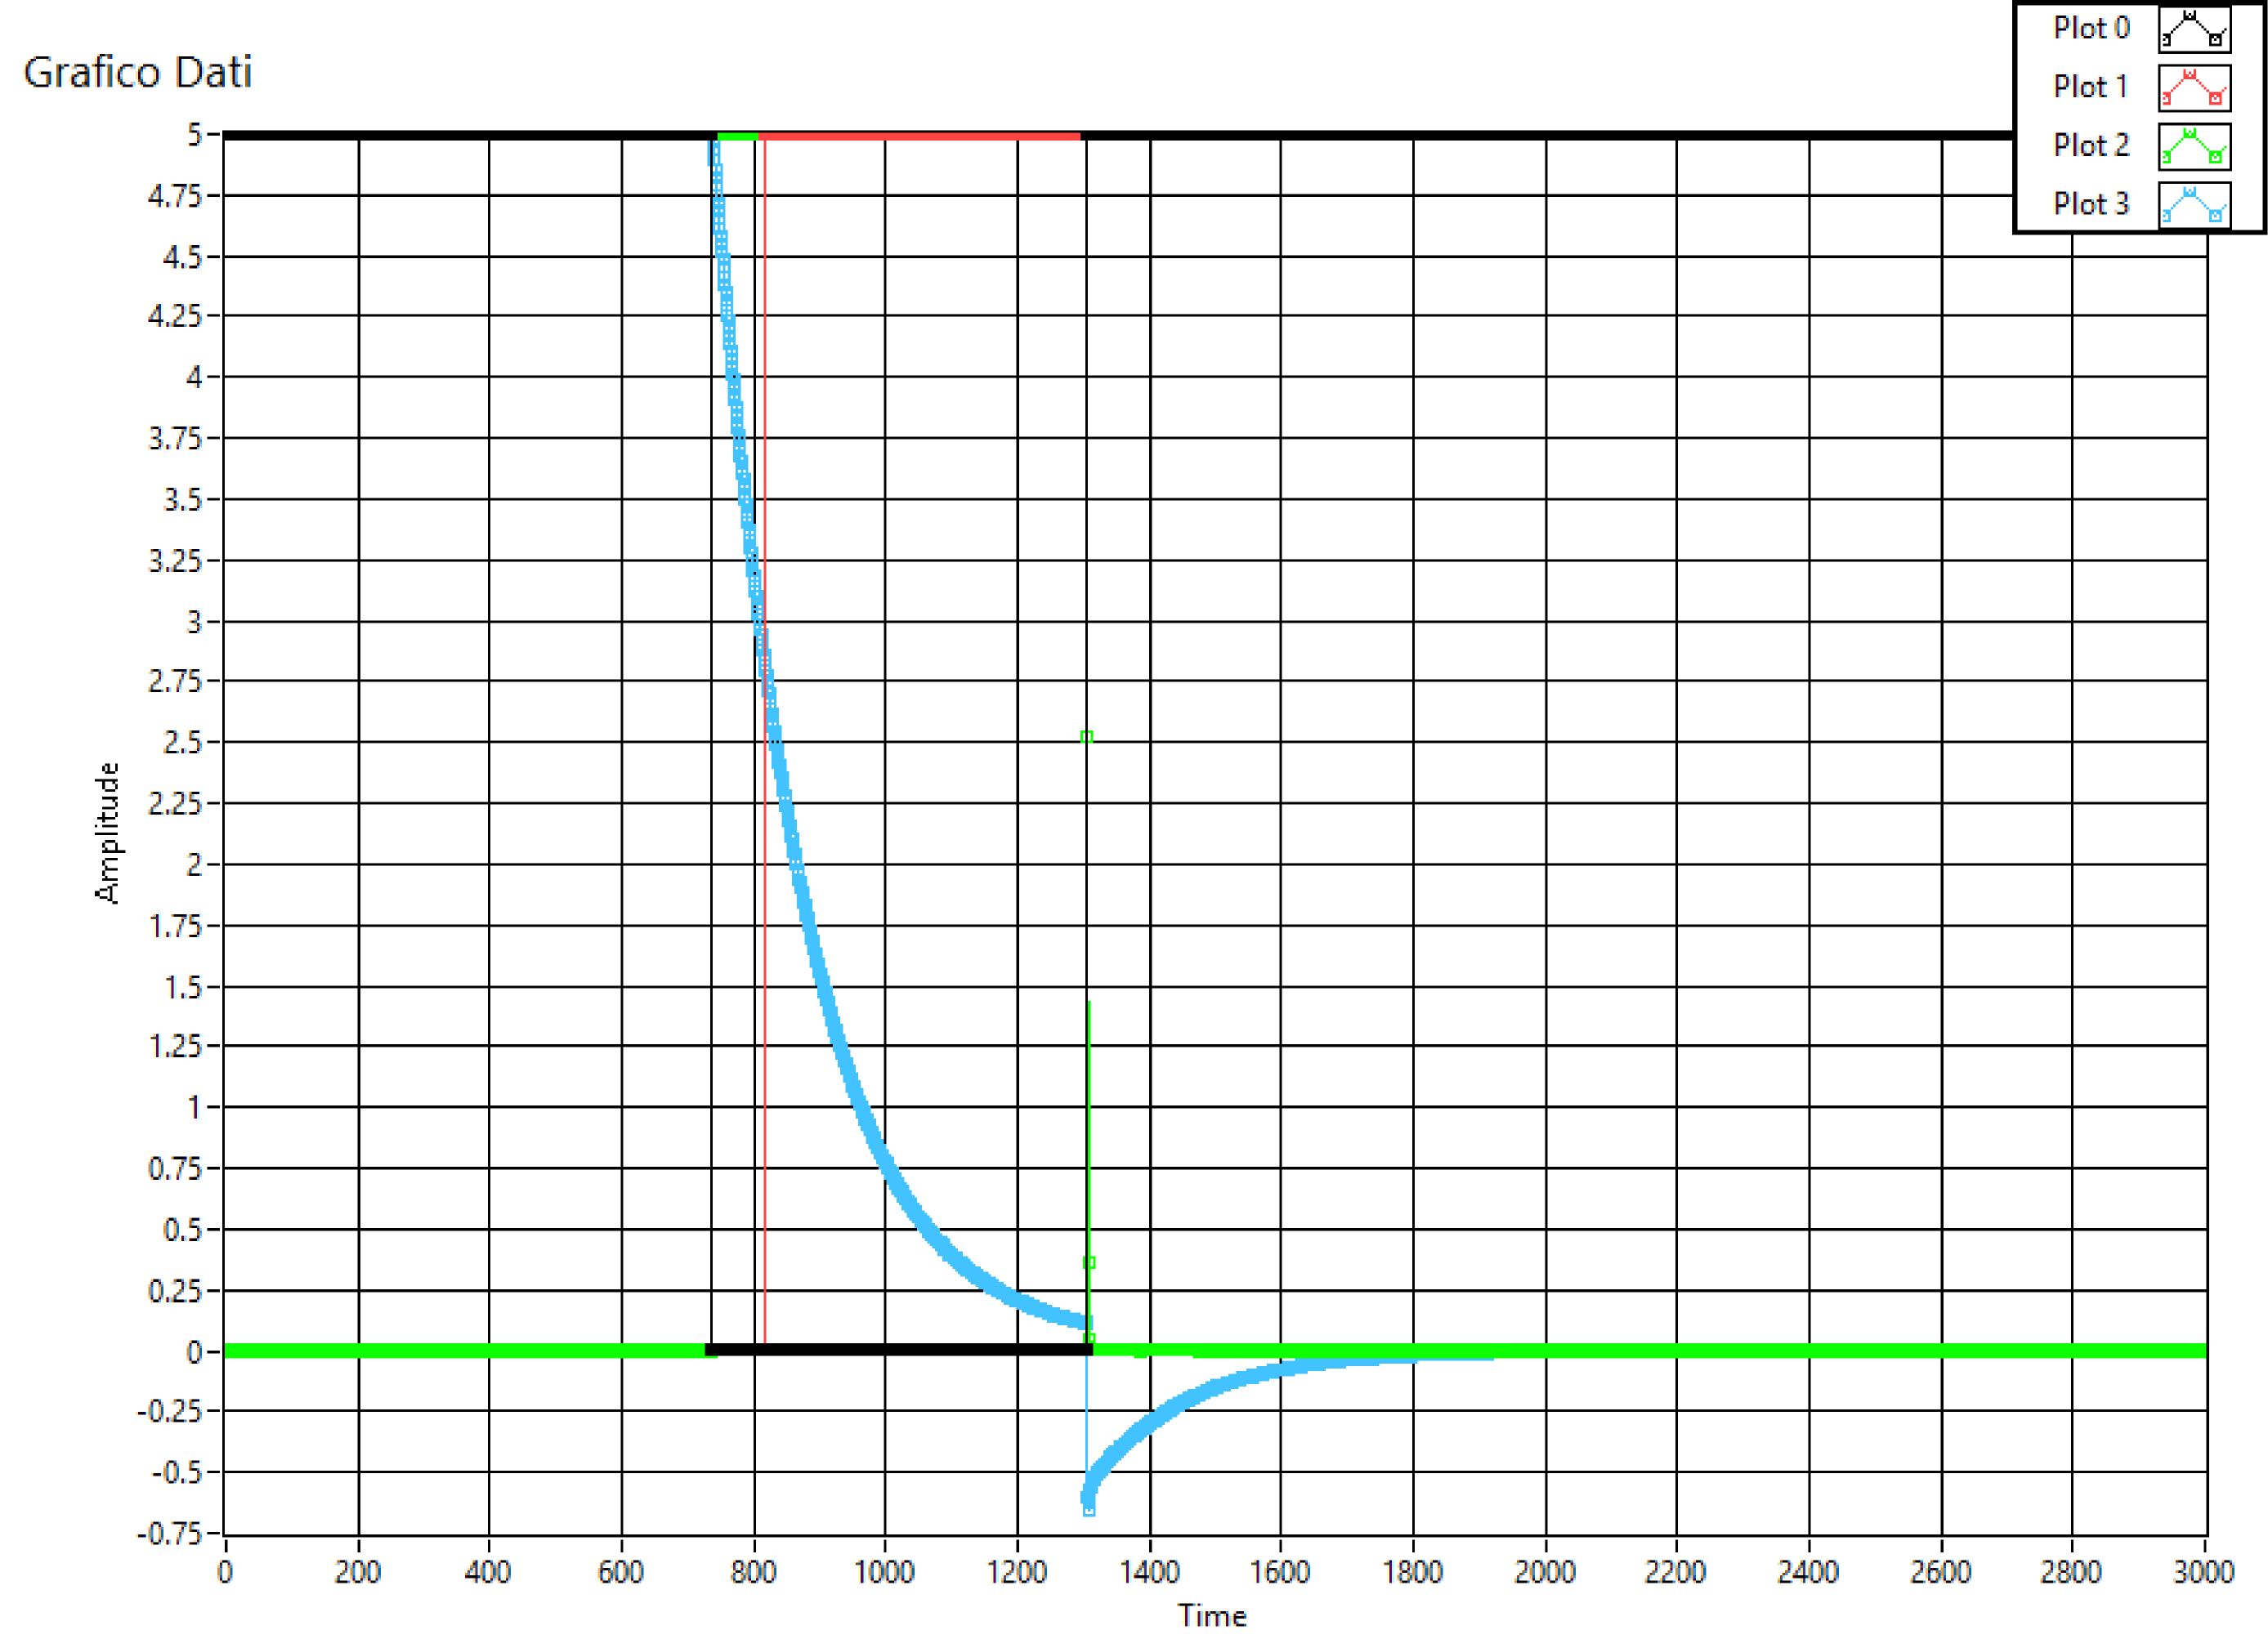
\includegraphics[width=0.7\linewidth]{./es6_150k}
\caption{Segnale dei quattro canali a R=150kOhm. In azzurro V1, in nero T, in rosso U2 e in verde U1.}
\label{fig:es6_150k}
\end{figure}

Riportiamo anche un grafico (vedi Figura (\ref{fig:es6_1MO_double})) per cui è stata impiegata una resistenza da 1M$\Omega$. Questa volta la durata dell'impulso negativo è di 544(1) ms, rispetto a quella prevista di $\sim 0.7 s$ (si ricordi che i dati aspettati sono affetti \underline{almeno} da un 10 \% di tolleranza dovuto all'incertezza sul condensatore).\\

\begin{figure}
\centering
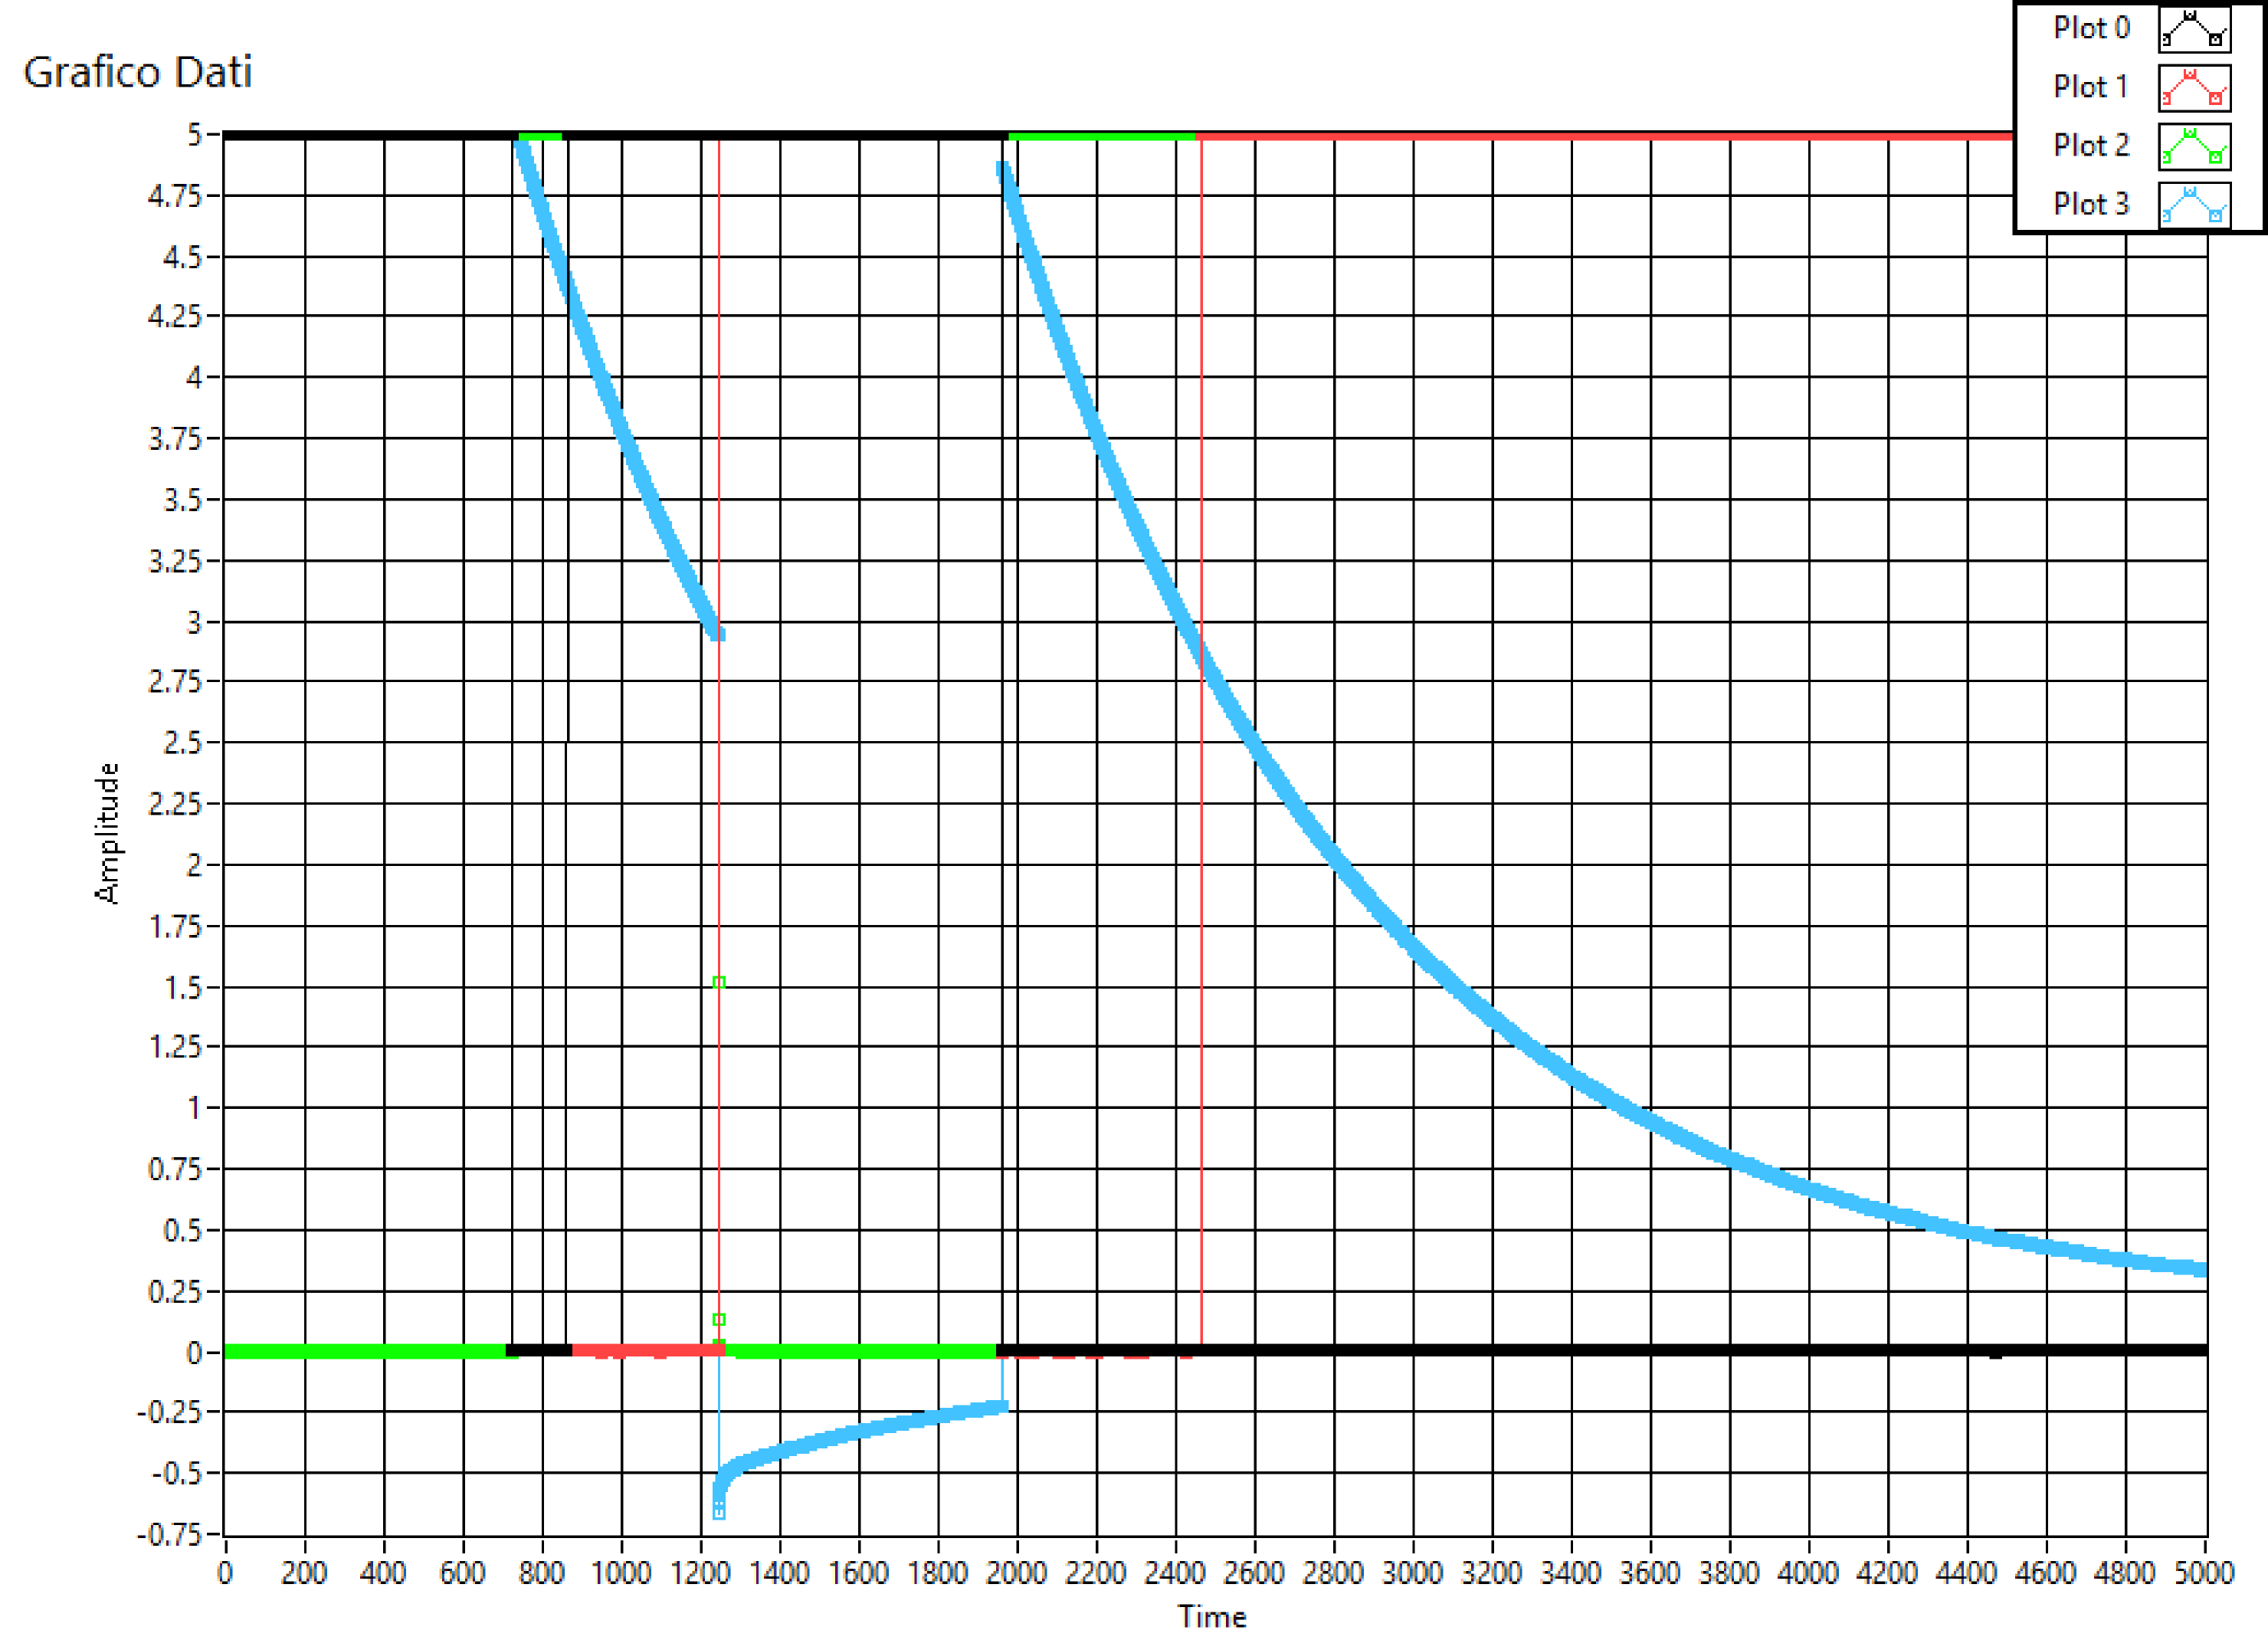
\includegraphics[width=0.7\linewidth]{./es6_1MO_double}
\caption{Segnale dei quattro canali del circuito metastabile, la legenda dei colori è la stessa per l'immagine precedente. La resistenza scelta è di 1MOhm.}
\label{fig:es6_1MO_double}
\end{figure}

Vogliamo ora ottenere una misura diretta della durata dell'impulso, tramite il \textsc{contatore\_pulsew}: utilizziamo lo stesso accorgimento di prima, vale a dire poniamo un \textbf{NOT} in serie a U2 e misuriamo quindi il \textit{rising time} con il VI (la resistenza scelta è da 150kOhm). Dobbiamo porre particolare attenzione alla frequenza che scegliamo al generatore come segnale di \textsc{clk}, poichè vogliamo evitare di retriggerare l'impulso (dato che a noi interessa a durata di un solo impulso singolo). Per questo motivo il periodo di clock deve essere certamente maggiore di 0.1s (a questo punto di 0.07s), il che corrisponde a frequenze minori di 10Hz (14 Hz). Purtroppo, il VI ha seri problemi ad acquisire segnali a frequenza così bassa, anche riducendo al minimo il numero di campionamenti (crasha continuamente). La minima frequenza che siamo riusciti ad acquisire è di 120Hz, con 7 campionamenti per avere una distribuzione semi-statistica. I risultati sono nella tabella che segue:\\


\begin{table}
\centering
\caption{tab\_es7}
\label{tab:es7}
{
\begin{tabular}{c|c}
\hline \textbf{frequenza} & \textbf{rising time} ms \\ 
\hline 120Hz & 61.58(5) \\ 
 150Hz & 61.04(5) \\ 
 200Hz & 60.16(3) \\ 
 500Hz & 52.87(3) \\ 
 1kHz & 29(5) \\ 
 5kHz & 7(3) \\ 
\hline 
\end{tabular}
}
\end{table}
~\\

Per ovviare a questo problema, abbiamo scelto una resistenza più bassa, da 47kOhm nominali, in modo che la durata dell'impulso si riducesse ($\tau_s \sim 0.033s$) e la frequenza massima si alzasse ($f_{max} = 30 Hz$). Questa volta siamo stati più fortunati e con il VI siamo riusciti a campionare anche frequenze di 1Hz. In generale, più è bassa la frequenza del \textsc{clk}, più il rising time si avvicina al tempo nominale caratteristico del circuito metastabile $\tau_s$. Stranamente, invece, all'aumentare della frequenza diminuisce il rising time, mentre invece ci saremmo aspettati che questo aumentasse (e che il duty cycle tendesse a 1) poichè entriamo in regime di retrigger continuo. (CAZZATA)\\

\begin{table}
\centering
\caption{tab\_es7bis}
\label{tab:es7bis}
{
\begin{tabular}{c|c}
\hline \textbf{frequenza} & \textbf{rising time} ms \\ 
\hline 1kHz & 8.3(5) \\ 
 500Hz & 16.04(2) \\ 
 200Hz & 18.08(2) \\ 
 100Hz & 18.07(5) \\ 
 10Hz & 22.35(1) \\ 
 8Hz & 22.76(2) \\
 5Hz & 23.51(1) \\
2Hz & 24.07(1) \\
1Hz & 24.10(1)\\ 
\hline 
\end{tabular}
}
\end{table}
~\\

Per esaminare meglio il retrigger di questa configurazione, usiamo il VI \textsc{digital\_pulse}, capace di generare una sequenza di impulsi della durata voluta e intervallati opportunamente. Consideriamo una resistenza di 470kOhm, per cui ci aspettiamo un $\tau_s = 0.33s$ (in analogia con la resistenza da 47kOhm precedentemente usata è più probabile che il tempo caratteristico sia di $\sim 0.24s$). Scegliamo un treno da 3 impulsi di 20ms ciascuno, intervallati da 100ms e registriamo l'uscita. Nel grafico in Figura (\ref{fig:es8_retrigger}) è riportato il risultato: durante la fase di "impulso negativo", il metastabile riceve altri 2 impulsi di trigger validi, tuttavia se andiamo a misurare la durata complessiva del impulso in uscita troviamo $\tau = 0.247(1)s$, che ci permette di affermare che il circuito è \textbf{non} retriggerabile.

\begin{figure}
\centering
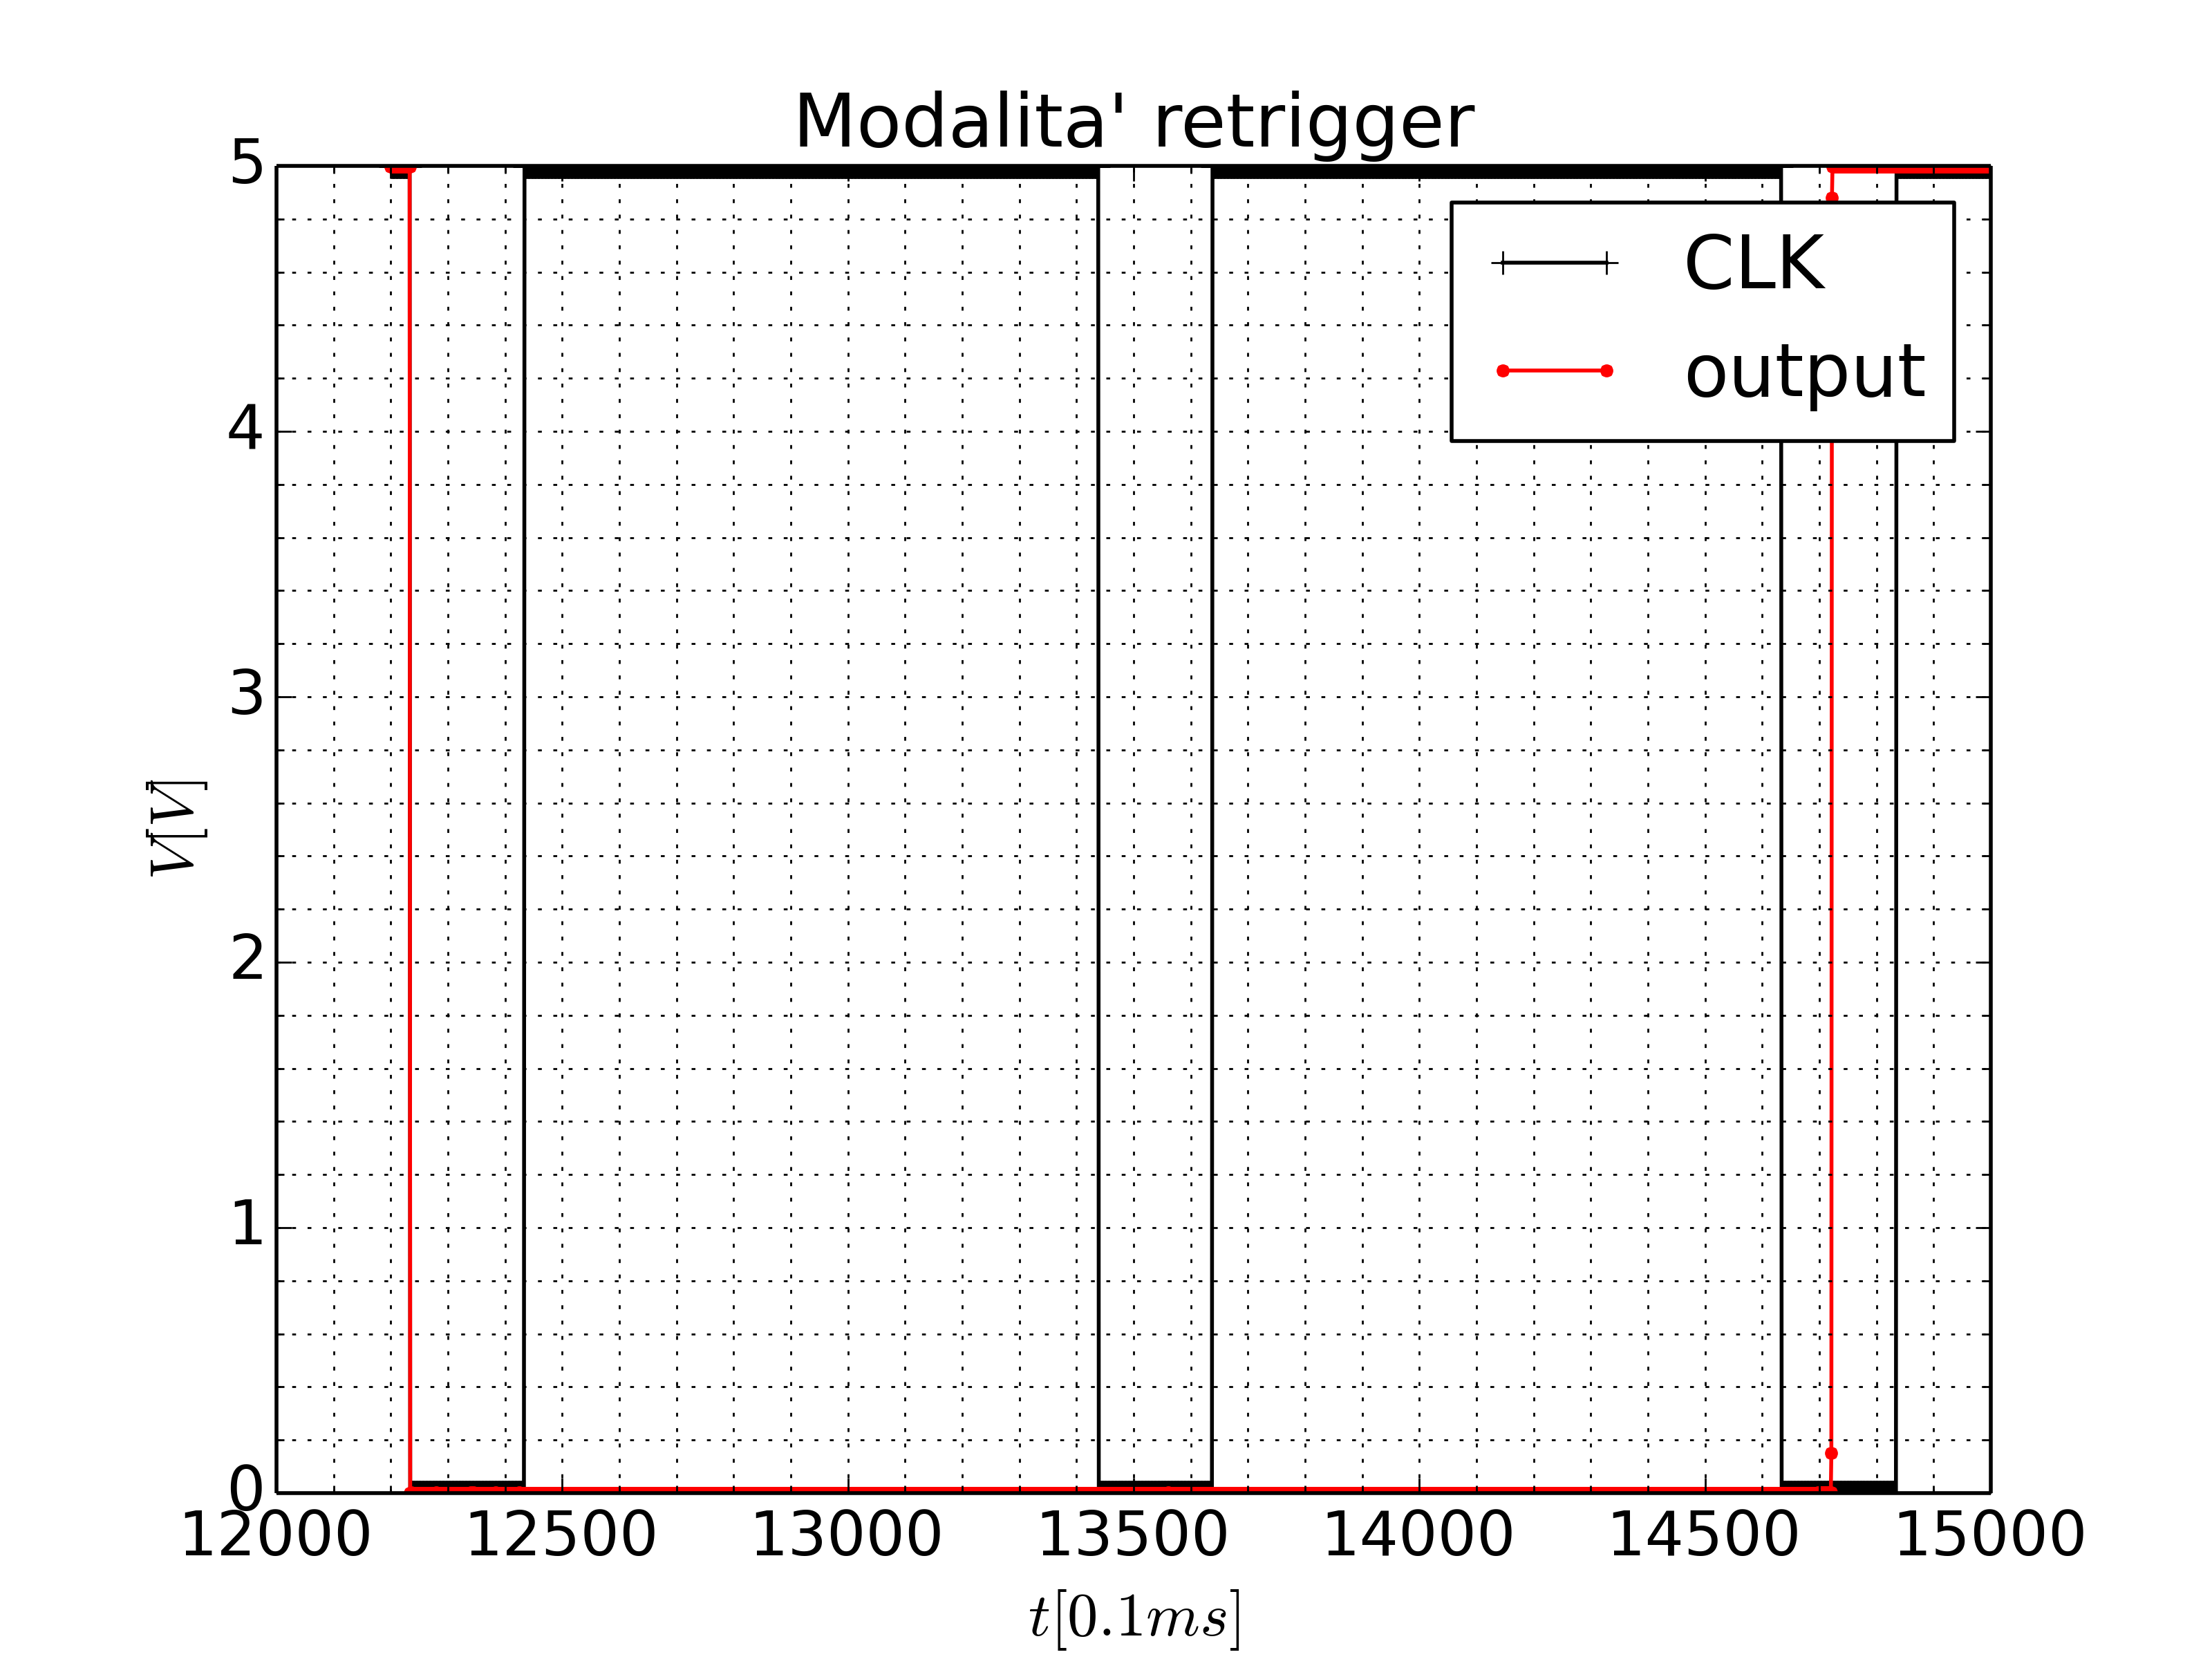
\includegraphics[width=0.7\linewidth]{./es8_retrigger}
\caption{Non-retriggerabilità del circuito metastabile: ricevendo ulteriori impulsi validi di trigger, la durata dell'impulso in output non varia.}
\label{fig:es8_retrigger}
\end{figure}

\section{Potenziometri digitali}
Abbiamo già avuto modo di usare il potenziometro (classico), vale a dire una resistenza variabile tramite la rotazione di una manopola. Questa volta siamo interessati a capire il funzionamento di un potenziometro digitale in cui, cioè, il valore di resistenza è selezionato mediante invio diun'opportuna sequenza di segnali digitali. Il potenziometro digitale da noi impiegato è il \textsc{NV trigger potentiometer ds1804} della Dallas Semiconductor. Dal datasheet fornito dal produttore ricaviamo alcune informazioni preliminari:

\begin{itemize}
\item E' un oggetto a 100 posizioni, quindi vi sono 100 passi selezionabili fra il valore minimo e quello massimo di resistenza;
\item opera a tensioni di 5V;
\item ha un'interfaccia di controllo di tipo up/down;
\item il modello da noi usato ha una resistenza massima di 10kOhm.
\end{itemize}

Dal datasheet, in particolare dalla Figura (), risulta che la selezione del valore di resistenza è fatta tramite un \textit{wiper} capace di posizionarsi in un punto preciso della serie di resistenze, in seguito a dei comandi sugli otto pin del potenziometro, che dunque determina una resistenza fra le uscite \textsc{high}-\textsc{wiper} e \textsc{low}-\textsc{wiper}. Il funzionamento base è quindi descritto dalla presenza di un \textit{multiplexer}, un oggetto che serve a collegare un gran numero di ingressi ad un numero ridotto di uscite (nel nostro caso una sola), commutando rapidamente fra tutte le linee di input.\\
Il controllo del dispositivo è dato da tre canali logici: il primo è il \textit{chip-select} $\neg CS$ che attiva (quando è zero), disattiva (quando è 1) la risposta a tutti gli altri segnali inviati al dispositivo.\\
In secondo luogo abbiamo il pin 2 che è chiamato up/down control: se questo è 1, lo spostamento del wiper avverrà verso il canale H, in caso contrario verso il canale L (fare riferimento alla Figura ()). Infine, ciò che determina lo spostamento del wiper è il segnale al pin 1, detto inc: ogni fronte di discesa provoca uno spostamento del wiper di una posizione verso H o L in base al valore di up/down.\\

\subsection{Hw. 2}
Ci chiediamo per quale motivo si ha effettivamente bisogno di un pin di tipo C/S che attiva o disattiva la ricezione degli altri segnali. Una possibile risposta che ci siamo dati è che questo permette una grande libertà nella selezione del valore della resistenza quando vi sono più potenziometri digitali collegati in parallelo (o anche in serie): disattivando o attivando C/S è possibile far muovere il wiper di solo alcuni fra i vari potenziometri, risparmiando un numero elevato di canali per il controllo individuale di ognuno.\\

Verifichiamo che il valore di resistenza sia compatibile con quello nominale: effettuiamo i collegamenti come mostrato in Figura (\ref{fig:es10circuit_export}) e colleghiamo un multimetro digitale in modalità ohmetro fra il canale H e il wiper: il valore restituito è di 9.97(8)kOhm.

\begin{figure}
\centering
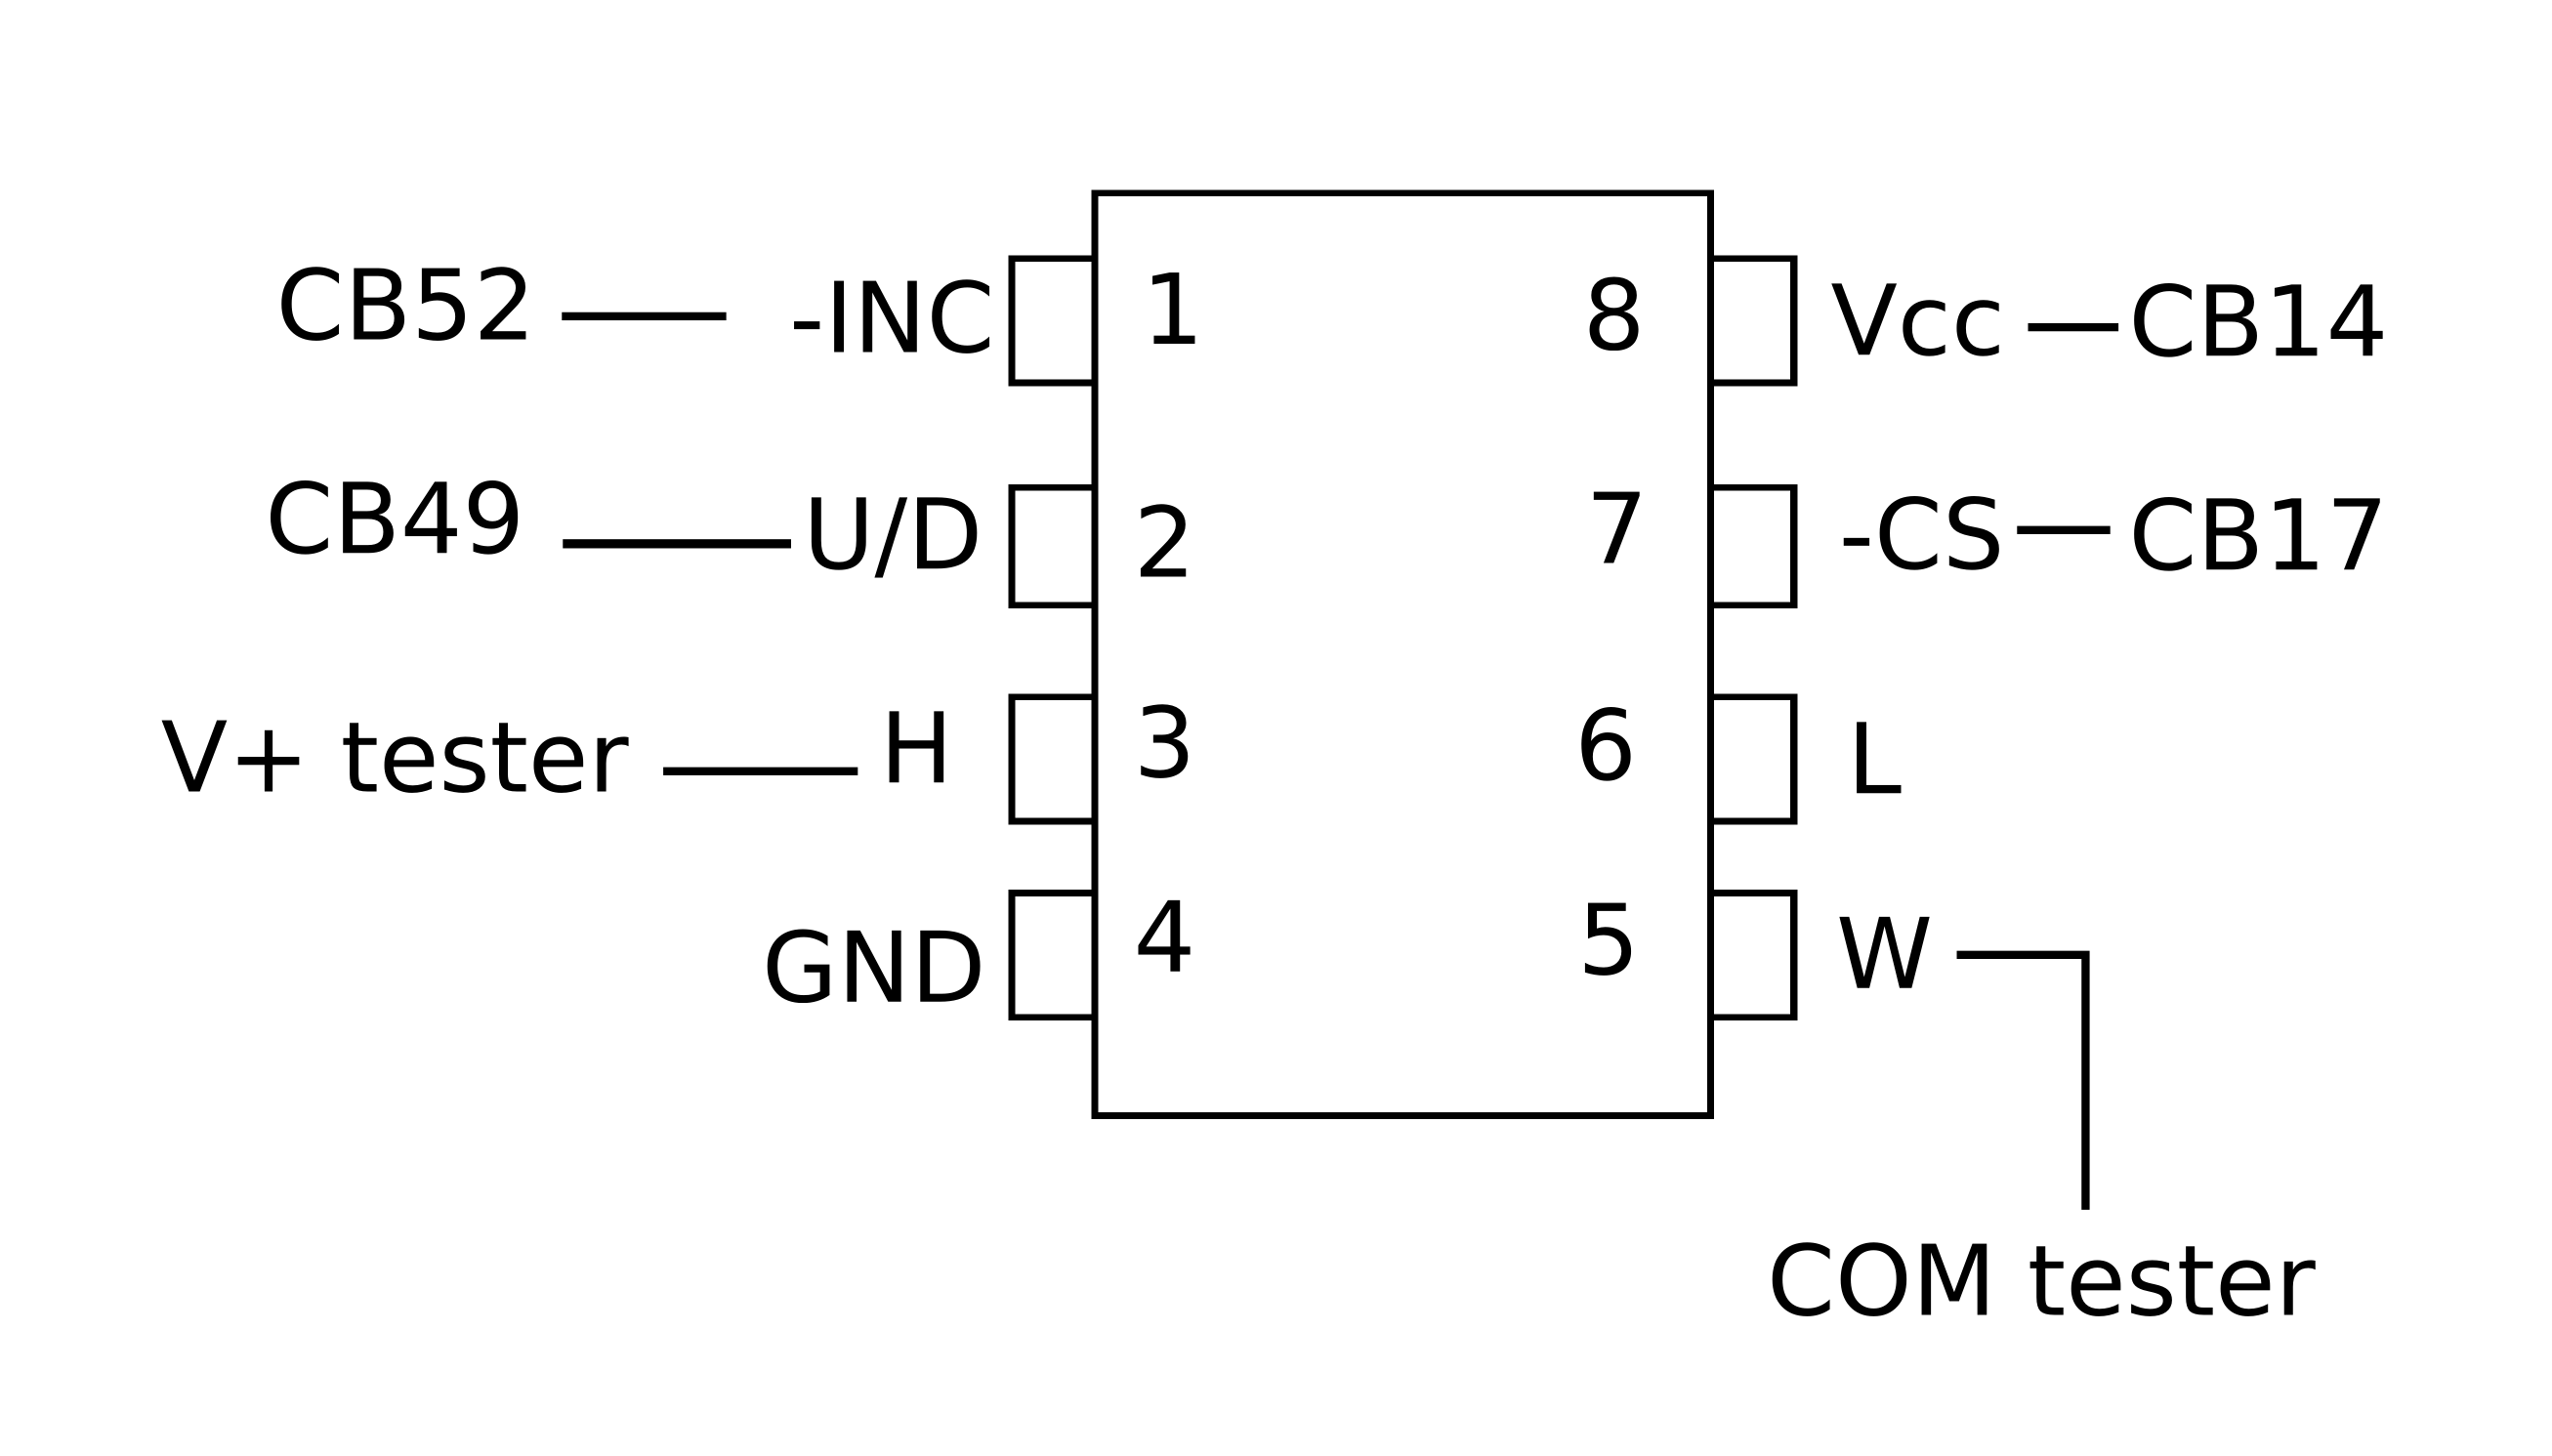
\includegraphics[width=0.7\linewidth]{./es10circuit_export}
\caption{Pin e collegamenti del potenziometro digitale}
\label{fig:es10circuit_export}
\end{figure}


\begin{thebibliography}{5}

	%Each item starts with a \bibitem{reference} command and the details thereafter.
	
	\bibitem{JH6} % Conference paper
	Product data sheet: Dual Type D Flip-Flop \textsc{mc14013b}.
	\url{http://onsemi.com}

	\bibitem{M06} % Conference paper
	Paul Horowitz, Winfield Hill - The Art of Electronics. Cambridge University Press (1989).
	
\end{thebibliography}


\end{document}